\chapter{関連研究}
関連研究や用語の定義,先行研究及びアプリケーションの先行事例を示す.

\section{時間管理の定義}
時間管理の定義は多岐にわたる.
例えば著名なものとしてLakeinの定義\cite{Lakein1989}の定義が挙げられる(表~\ref{tb:Lakein}).
Lakeinは個人管理という位置付けで時間管理に言及し,下記の4項目に則り時間管理を遂行していく重要性を説いた.

\begin{table}[htb]
\begin{center}
  \begin{tabular}{|l|l|} \hline
   1 & すべきことを決定する \\ \hline
   2 & 達成するための目標を設定する \\ \hline
   3 & 優先順位を決める \\ \hline
   4 & 取り組む課題のプランニングを作る \\ \hline
  \end{tabular}
  \caption{Lakeinによる時間管理の定義}
  \label{tb:Lakein}
\end{center}
\end{table}

Claessens et al. は,先行研究の定義を俯瞰した上で,時間管理を"目標を達成するために時間を効果的に使用する行動"と定義し時間管理の行動を更に以下の3つに分類した\cite{Claessens2007}(表 ~\ref{tb:Claessens}).

\begin{table}[htb]
\begin{center}
  \begin{tabular}{|l|l|} \hline
   時間アセスメント行動(time assessment behavior): \\ ~~~過去,現在,未来の時間を認識し,時間の使い方に関して認識する事 \\ \hline
   プランニング行動(planning behavior): \\  ~~~時間を効率的に使用する事を目的とする事 \\ \hline
   モニタリング行動(monitoring behavior): \\ ~~~行動中における時間の配分のモニタリング・不測の事態へのリスクヘッジ等 \\ \hline
  \end{tabular}
  \caption{Claessens et al. による時間管理の定義}
  \label{tb:Claessens}
\end{center}
\end{table}

\section{時間管理の先行研究について}
時間管理研究は大きく分けて時間管理がもたらす効果の研究と時間管理能力に関する研究の2種類に分けられる.
時間管理能力の研究では主に見積もり時間の精度に関して議論されている.
見積もりの精度は大きく分けて課題に対するもの\footnote{与えられた課題の時間 \cite{Roy2008}や経験の有無\cite{Roy2007}}と被験者の個人差によるもの\footnote{時間評価における知覚時間の歪み\cite{Oguro1961}\cite{Murakami2016}}の2種類存在しているが,
原因として記憶との関連性が考えられている\cite{Roy2005}.

正確な見積もりを計算する手法は主に大規模プロジェクト向けに提案される事が多い.
例えばPERT(Program Evaluation and Review Technique)では個々のタスクの見積もりを予測する手法である「三点見積もり法」が考案されている.
タスク完了に要する時間の最良見積もり(期待時間)値を$T_{E}$,タスク完了に必要な最小時間の予測(楽観的時間)を$O$,タスク完了に必要と思われる最頻値の見積時間(最確時間)を$M$,タスク完了に必要な最大時間の予測(悲観的時間)を$P$とすると,数式(\ref{pert})の様に見積もりを行う\footnote{ただし,三点見積もり法は参加者が複数人いる長期の大型プロジェクトに対する適切な管理方法であり,参加者の多くないプロジェクトでは最可能値だけを使用した見積りのほうが正確である場合がある\cite{Kato1965}}.
\begin{equation}
\label{pert}
T_{E} = (O + 4M + P) ÷ 6
\end{equation}

\section{時間管理の評価方法}
代表的な時間評価の方法としては,被験者に時間の長さを教示し,その長さを産生させる時間産生法(時間作成法)(time production),
被験者が時間を経験した後に体験時間を再生させる時間再生法(time reproduction),
経過した時間間隔を言語的に評価する言語的時間評価法(verbal timeestimation)などがある\cite{Oguro1961}\cite{Tayama2018}.

\section{日常生活動作、及び個人管理としての時間管理}
日常生活動作(Activities of Daily Living;ADL)とは,人が日常生活において繰り返す,身の回りの活動や動作のことである.具体的には,身の回りの動作(食事,更衣,整容,排泄,入浴の各動作),移動動作,その他生活関連動作(家事動作,交通機関の利用等)を指す\cite{Sakai2003}.
今日では特にパフォーマンスやストレスなど様々な観点から個人管理面においても適切な時間管理が求められている.\cite{Barling1996}\cite{Britton1991}\cite{Burt1994}\cite{Macan1994}.

\section{時間管理をサポートするシステムの分類}
今日,日常生活動作を基調とし,身近な時間管理をサポートするシステムが複数開発されている.
まず,身近な時間管理をサポートするシステムにはトップダウン式のものとボトムアップ式のものがある.
トップダウン式は予め秒数が固定されたルーティンに沿って時間を遂行する事を補助するものであり,
例えばルーチンタイマー\cite{RoutineTimer} (図~\ref{fig:routine})やポモドーロテクニック\cite{pomodoro} などが挙げられる,
\\
\begin{figure}[ht]
\begin{center}
\begin{tabular}{c}
  	\begin{minipage}[b]{0.5\linewidth}
	\begin{center}
		\fbox{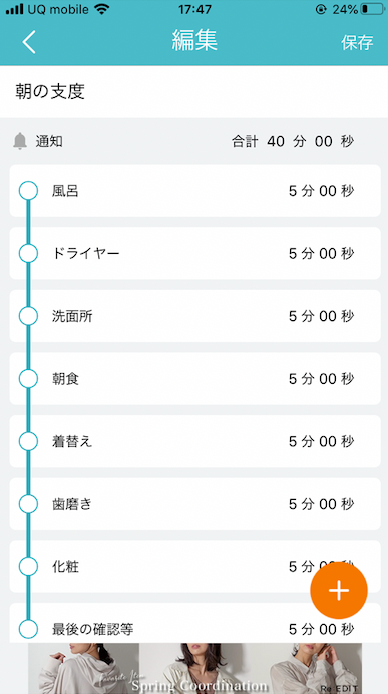
\includegraphics[width=5cm]{images/2/routine.png}}
		\caption{ルーチンタイマーの行動設定例}
		\label{fig:routine}
	\end{center}
  	\end{minipage}
\end{tabular}
\end{center}
\end{figure}
\\
一方,ボトムアップ式は時間の使い方を可視化する事を主眼としているものである.

ボトムアップ式の時間管理システムは図~\ref{fig:bottomup}の様に大別が可能である.
\begin{figure}[ht]
\begin{center}
\begin{tabular}{c}
  	\begin{minipage}[b]{0.5\linewidth}
	\begin{center}
		\fbox{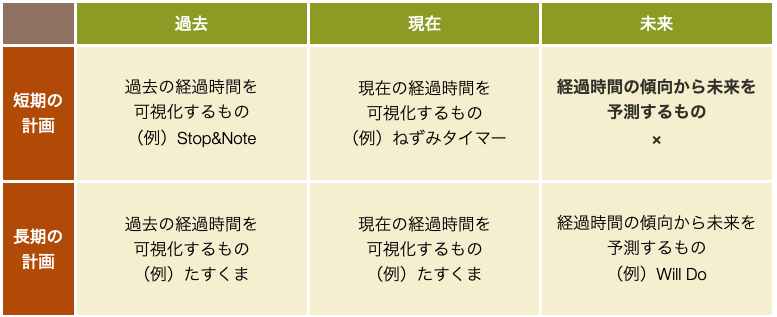
\includegraphics[width=12cm]{images/2/bottom.png}}
		\caption{ボトムアップ式の時間管理システムに関する分類}
		\label{fig:bottomup}
	\end{center}
  	\end{minipage}
\end{tabular}
\end{center}
\end{figure}
まずは行動をタスク別に計測を行う事で過去自分の使った時間を記録し,可視化する事で振り返りに役立てるシステムである.
例えばストップウォッチとメモ帳を組み合わせたStop\&Note\cite{pomodoro}や日毎の時間傾向を可視化するたすくま\cite{Taskuma}(図~\ref{fig:taskuma}))といったシステムが挙げられる.
次に,ある時間からの経過時間を可視化する事によって現在の経過時間把握を補助するシステムである.
所謂ストップウォッチは勿論の事,例えば時間の流れをイラストで表現するもの(ねずみタイマー\cite{MouseTimer}(図~\ref{fig:mouse}))や時間把握の精度をミニゲームに昇華させたもの\cite{JUSTTIME}などが挙げられる.
\begin{figure}[ht]
\begin{center}
\begin{tabular}{c}
  	\begin{minipage}[b]{0.5\linewidth}
	\begin{center}
		\fbox{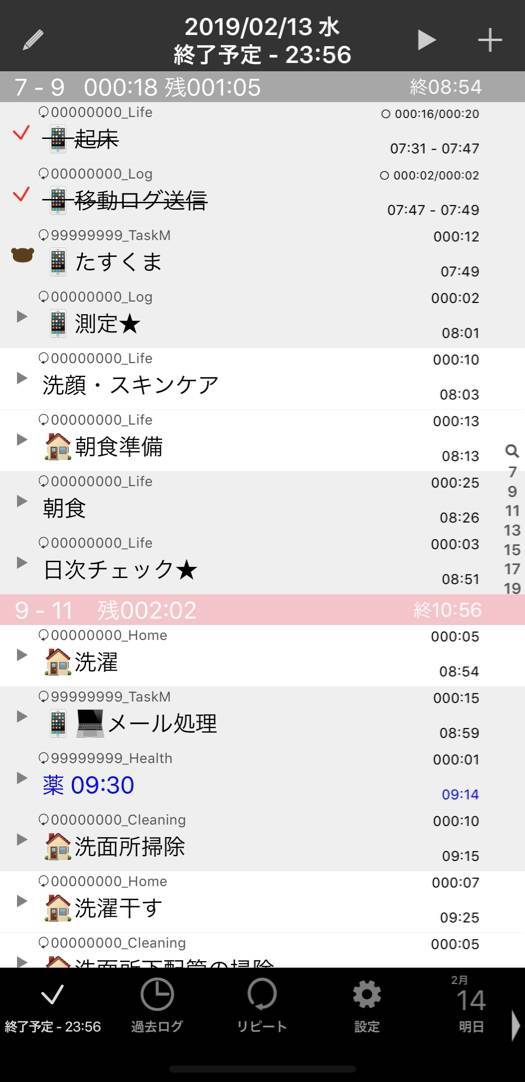
\includegraphics[width=5cm]{images/2/taskuma.png}}
		\caption{たすくまによる一日の可視化}
		\label{fig:taskuma}
	\end{center}
  	\end{minipage}
\\
  	\begin{minipage}[b]{0.5\linewidth}
	\begin{center}
		\fbox{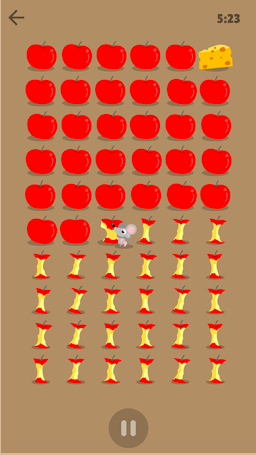
\includegraphics[width=5cm]{images/2/mouse.png}}
		\caption{ねずみタイマーによる経過時間の可視化}
		\label{fig:mouse}
	\end{center}
  	\end{minipage}
	
	\begin{minipage}[b]{0.5\linewidth}
	\begin{center}
		\fbox{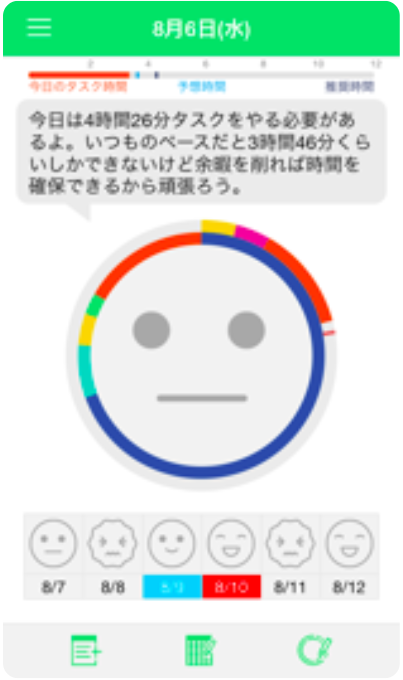
\includegraphics[width=5cm]{images/2/willdo.png}}
		\caption{WillDoによる未来予測}
		\label{fig:mouse}
	\end{center}
  	\end{minipage}
\end{tabular}
\end{center}
\end{figure}

最後に,行動をタスク別に計測する事によって自分の時間傾向をシステム側が把握し,未来自分がどうなるかを予測するシステムである.
この方向性を持つシステムは現在限られているものの,例えばWillDo\cite{willdo}(図~\ref{fig:taskuma}))が挙げられる.
WillDoは一日の行動を記録することによって,特定のプロジェクトが目標達成までに毎日どれだけかけるべきかを提示する.
\section{まとめ}
本章では,本研究における関連研究を整理し,問題意識を洗い出した.
次章では,筆者が本研究に先立ち行った研究について述べ,問題意識を洗い出す.